\section{Code Size}

This section looks at the size of the compiled object files for various {\rust} libraries and runnable programs.
A comparison between functionally equivalent programs in {\C} and {\rust} is provided.

Code size is an important factor in an embedded system.
The systems are more restricted than conventional systems especially when it comes to storage.
For the EFM32 line of microcontrollers the code is stored in flash memory.
In \autoref{sec:back:hw} we showed that the flash memory in the EFM32 family of microcontrollers ranges from 4KB to 1MB.
As \autoref{sec:before-main} explains the flash memory should not only contain the program code but also the constant data defined in the program.
This limits the code size even further.

Another concern which makes code size a priority in embedded system is price.
When putting an embedded system into production, the number of microprocessors is usually large.
And as the size of the flash correlates with the price of the microprocessors, being able to choose a smaller version can save large amounts of money.

Each program was compiled with optimization levels O0, O1, O2 and O3, the O0 level is compiled both with and without debugging symbols.
Compiling the library results in a \file{lib*.rlib} file which is an archive containing object files for the code contained in the library.
Compiling executable programs results in an {\elf} binary file.
The size is then calculated by executing the \emph{arm-none-eabi-size} program.

\subsection{Measuring Size}
\label{sec:measure-size}

The \emph{arm-none-eabi-size} program accepts an elf binary, an object file or an archive as argument.
The program then reads the file and reports the size of the \elfsec{.text}, \elfsec{.data} and \elfsec{.bss} segments, described in \autoref{sec:back:elf}.
If the argument is an archive, the program will iterate through all the objects in the archive and report the size for each individual object file.
When reporting the size of the archives, the sizes for all the objects files contained within the archive have been accumulated.

\subsection{Parameters}
\label{sec:size:params}
The various files where compiled by setting the compiler optimization flags in the \file{Cargo.toml} file.
The parameters used are shown in \autoref{tab:size:params} with their effect.

\begin{table}[H]
  \centering
  \begin{tabular}{l|l|l}

    \textbf{Parameter} & \textbf{Values} & \textbf{Effect} \\
    \hline
    debug & true, false & sets the \textbf{-g} flag on the compilers  \\
    debug-assertions & true, false & a way to remove assertion statements \\
    opt-level & 0, 1, 2, 3 & sets the optimization flag on the compilers \\
    lto & true, false & sets the Link Time Optimization flag on the linker \\
    \hline
  \end{tabular}
  \caption{Cargo.toml parameters and their effect}
  \label{tab:size:params}
\end{table}

Each program in this section is compiled with 6 different settings as given by \autoref{tab:size:settings}.
\begin{table}[H]
  \centering
  \begin{tabular}{l|l|l|l|l|l|l}
    & \textbf{1} & \textbf{2} & \textbf{3} & \textbf{4} & \textbf{5} & \textbf{6} \\
    \hline
    debug            & true  & false & false & false & false & false \\
    debug-assertions & true  & false & false & false & false & false \\
    opt-level        & 0     & 0     & 1     & 2     & 3     & 3     \\
    lto              & false & true  & true  & true  & true  & true  \\
    (c code Os)      & false & false & false & false & false & true \\
    \hline
  \end{tabular}
  \caption{Compilation settings}
  \label{tab:size:settings}
\end{table}

Notice that for the 6th optimization setting, the underlying {\C} sources is compiled with the Os flag.
For the rest of the settings the same optimization level is used for both the {\rust} and the {\C} code.
This 6th optimization setting is only used when compiling binaries.

\subsection{Libraries}

We first look at the code size of the \gls{rel} libraries along with the \lib{cmsis} and \lib{startup} libraries.
The \gls{rel} libraries, presented in \autoref{sec:rel}, all contain {\rust} code only, while the \lib{cmsis} and \lib{startup} libraries contain {\rust} binding code in addition to the actual {\C} implementation code compiled with \prog{gcc}.
The same compiler options from \autoref{sec:size:params} are passed to the {\C} compiler.
As the code size of libraries varies from a few bytes to 400KB,the results are presented in two separate figures.
\autoref{fig:size:lib:small} shows the small libraries ranging from 4B to 3KB and \autoref{fig:size:lib:large} shows the large libraries in ranges 100KB to 400KB.

The \prog{arm-none-eabi-size} makes the distinction between three of the {\elf} segments.
Here, only the size for the \elfsec{.text} segment are shown in the graphs, as the \elfsec{.data} and \elfsec{.bss} are mostly non-existing.
This is because there is not any static allocation in \gls{rel}, in fact the only static allocation is of 8B in the \textbf{data} section of the \lib{startup} library.

The bars for each library from left to right represent the sizes of programs compiled with different parameters as described in \autoref{tab:size:settings}.
The general trend is that the code size decreases as the optimization level is increased.

\begin{figure}[H]
  \begin{center}
    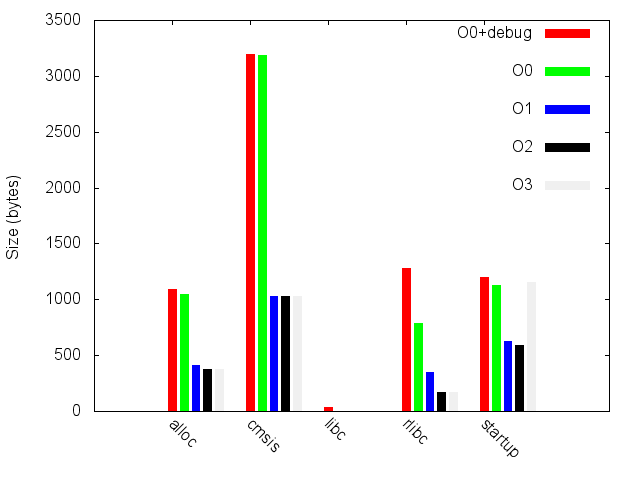
\includegraphics[scale=0.5]{results/plots/size/lib/small/size.png}
  \end{center}
  \caption{Code size for small Rust libraries}
  \label{fig:size:lib:small}
\end{figure}

A notable result in \autoref{fig:size:lib:small} is the increase in code size for the \lib{startup} library when moving from O2 to O3.
This increase of 500B is not due to the {\rust} code of the \lib{startup} library, but the \gls{cmsis} Cortex-M3 System Layer provided by Silicon Labs, and written in {\C}.

\begin{figure}[H]
  \begin{center}
    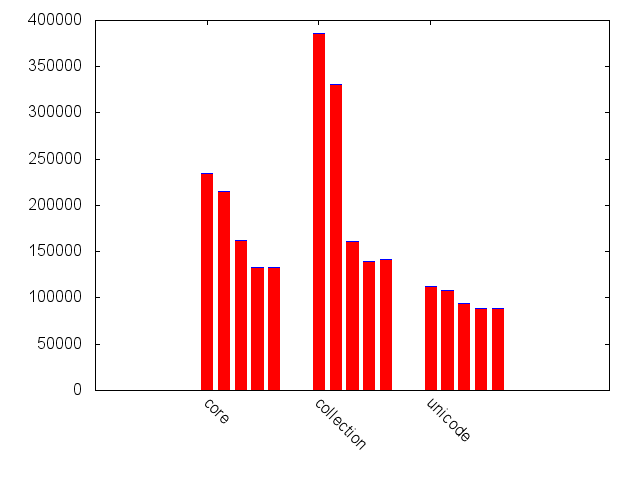
\includegraphics[scale=0.5]{results/plots/size/lib/large/size.png}
  \end{center}
  \caption{Code size for large Rust libraries}
  \label{fig:size:lib:large}
\end{figure}

From \autoref{fig:size:lib:large} we see that the \lib{collection} library is the largest one at ~137 KB when optimized.

%\todo{Move to discussion}
%\autoref{fig:size:lib:large} shows that some of the central libraries in \gls{rel} are quite large.
%An important point here is that, although the \lib{core} library by itself is over 100KB, when optimized for an actual program utilizing the library, it can be substantially smaller.
%This is because of the fact that a library build must provide all the functionality of the source code, while an executable build can eliminate all the functionality of the library that is not used.

\subsection{Executables}

This subsection consider the code size of actual runnable programs.
Functionally equivalent versions are written in both {\rust} and {\C} and here we compare the size of the binaries produced at each optimization level presented in \autoref{tab:size:settings}.
For the {\C} program an additional optimization level, -Os, is given as the rightmost bar.
This level tells the compiler to optimize for code size, it is not available for the {\rust} compiler at time of writing.
The first figure, \autoref{fig:size:bin:large}, in this section looks at the size of binaries generated for the two projects described in \autoref{sec:projects}.

\begin{figure}[H]
  \begin{center}
    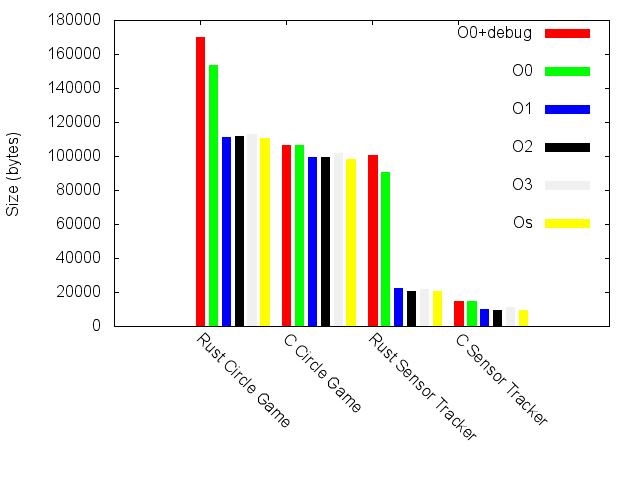
\includegraphics[scale=0.5]{results/plots/size/bin/large/size.png}
  \end{center}
  \caption{Code size for Project binaries}
  \label{fig:size:bin:large}
\end{figure}

The same trend as for the Libraries is seen for the {\rust} programs, higher optimizations levels provides a smaller binary.
Notice we see that the O2 level provides a small size gain over the O3 version.

The {\C} code does not exhibit the same size loss when optimized and the Os level builds produces consistently the smallest binary.

\autoref{fig:size:bin:small} shows the code size of a minimal program to boot the Gecko.
Both implementations only contain an infinite loop and are evaluate to examine the overhead of the languages.

\begin{figure}[H]
  \begin{center}
    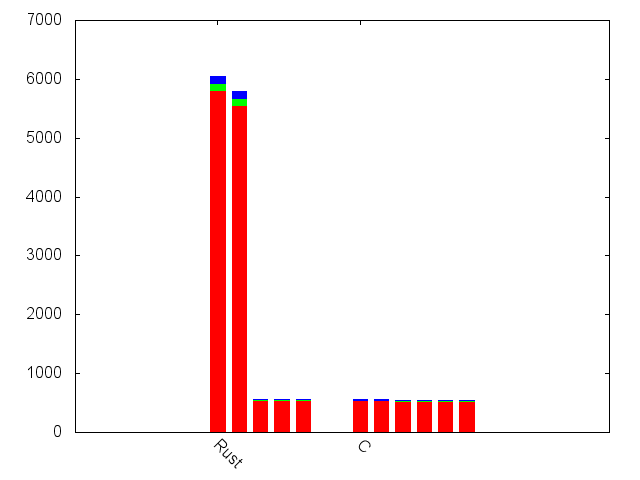
\includegraphics[scale=0.5]{results/plots/size/bin/small/size.png}
  \end{center}
  \caption{Code size for minimal program}
  \label{fig:size:bin:small}
\end{figure}

As explained in \autoref{sec:impl:booting} {\rust} does not require any additional initialization or setup compared to {\C}.
This is evident in \autoref{fig:size:bin:small} where the binaries are the same size when applying optimizations.
The debug and unoptimized {\rust} build is 10x lager compared to the optimized version.

\autoref{tab:size:c-vs-rust} compares the size of the smallest {\C} and {\rust} binaries for each of the evaluated programs.
The number reported is generated by dividing the size of the {\rust} binary by the size of the {\C} binary, giving the factor of which the {\rust} version is larger than the {\C} version.

\begin{table}[H]
  \centering
  \begin{tabular}{|c|c|c|}
    \hline
    {\cg} & {\tracker} & Minimal Main \\
    \hline
    1.22x & 2.20x & 1.03x \\
    \hline
  \end{tabular}
  \caption{{\rust} code size relative to {\C}}
  \label{tab:size:c-vs-rust}
\end{table}

We see from \autoref{tab:size:c-vs-rust} that both the {\cg} and the Minimal Main  {\rust} binaries come quite close to the {\C} binaries in size.

In \autoref{tab:size:breakdown} we break down of the size of the optimized build of the {\tracker}, too see which portions of the {\rust} code that make the binary size increase.

\begin{table}[H]
  \centering
  \begin{tabular}{l|r|r|l}
    \textbf{Section}      & \textbf{C (B)} & \textbf{Rust (B)} & \textbf{Relative} \\
    \hline
    \textbf{app}          & 1776 & 3964 & 2.23x \\
    \textbf{binding}      & 0    & 184  & N/A  \\
    \textbf{emlib}        & 4348 & 4376 & 1.01x \\
    \textbf{REL}          & 0    & 3516 & N/A  \\
    \textbf{newlib}       & 2372 & 792  & 0.33x \\
    \textbf{system}       & 460  & 896  & 1.95x \\
    \textbf{unwind}       & 0    & 3820 & N/A  \\
    \hline
  \end{tabular}
  \caption{Break down of binary sizes for {\tracker} application}
  \label{tab:size:breakdown}
\end{table}

In \autoref{tab:size:breakdown} we see that there are three major non-constant contributors\footnote{The \textbf{system} section increased with $\sim$2x, but this section will remain constant as the complexity of the application increases.} to the increased size for the {\rust} binary:

\begin{itemize}
\item The application
\item Rust Embedded Library
\item {\rust} expection mechanism (unwind)
\end{itemize}

We see that the \lib{newlib} implementation is reduced in the {\rust} binary.
This is due to the \gls{rel} library implementing some of the same functionality as \lib{newlib}, thus the this part of the \lib{newlib} is not included.

%\subsection{Discussion}

%This section has shown that the code size of all {\rust} binaries are larger than their {\C} counterparts.
%The optimized {\rust} builds does come close to {\C} builds with being 1.94x larger on average, while the debug builds are far bigger, 6.88x on average.

%The test hardware used to produce the results given here is the EFM32GGF1024, as mentioned in \autoref{sec:back:hw}.
%This chip has 1MB for storing the code and therefore running the debug builds which maxed out at ~176KB, was not a problem.

%Considering the Minimal Main debug binary presented in \autoref{fig:size:bin:small} and comparing to the chips with lower specifications in the EFM32 family (\autoref{tab:efm32-family}), we see that a debug build can not be executed at small versions of the Zero and Tiny Gecko.
%Looking at the {\tracker} application, even the heavily optimized version of the {\rust} build can not run on the largest version of the either the Zero or Tiny Gecko.

%Reading the results presented here should take in mind that the comparisons are made between a mature production proven compiler \textbf{gcc} and a pre/close to 1.0 compiler \textbf{rustc}.
%The design objectives for the 1.0 version of {\rust} as outlined in \autoref{sec:rust:roadmap} has been on stabilizing the language APIs and features.
%This indicates that non-breaking changes like compiler optimizations both for compiler speed and binary code sizes not has been a priority leading up to the 1.0 release.
